\chapter{Analisi di sensitività}
\label{chap:ansens}
Sulla base del modello descritto al capitolo precedente sono state sviluppate diverse analisi di sensitività rispetto alle variabili che determinano il valore del modello proposto. Tali simulazioni, univariate, realizzate tramite il programma di calcolo \textit{MATLAB}\footnote{I codici del programma creato sono riportati nell'appendice \ref{app:listatomatlab}.}, si basano sulla simulazione di variazioni (o \textit{shock}) sulle variabili ritenute di maggior impatto sul valore finale. Nei paragrafi che seguono sono riportati in sintesi i principali risultati, disponibili anche in valore assoluto (espressi in euro) nell'appendice \ref{app:risultati}.

\section{La sensitività dei flussi di cassa}
\label{sec:simvcf}
L'analisi della dipendenza del modello dei \textit{DCF} dai {\itshape cash flows}, ovvero dal livello delle entrate attese, si sviluppa in due direzioni: la prima simulazione prende in considerazione una variazione limitata ai soli affitti, la seconda  ipotizza che la variazione coinvolga anche l'ammontare finale a cui si stima di vendere l'immobile.
Ad una prima impressione la prima simulazione può sembrare superflua o almeno parzialmente distante dalla realtà del mercato immobiliare, tuttavia lo scenario simulato non è improbabile, ancorchè raro. Un esempio in tal senso può essere l'ipotesi di una bolla speculativa che all'ultimo periodo faccia rivalutare l'immobile, o meglio rimuova il fattore di shock. Un altro caso che trova applicazione nella prima simulazione è quello descritto dalla teoria del cosiddetto {\itshape greater fool} (\cite[p. 203]{geltner}), teoria secondo la quale un investimento frutto di una valutazione errata potrà essere \textit{ceduto} ad un più grande \textit{fool} presente sul mercato.
Le simulazioni svolte ipotizzano shock progressivi in base 5\% con una magnitudo del 25\% del valore, sia per gli scenari positivi che per quelli negativi. La misura della magnitudo deriva dalle specifiche tecniche riportare per il {\itshape property risk} all'interno dei documenti tecnici dell'EIOPA in merito al {\itshape QIS 5} (\cite[p. 174]{qistechnical}).

\subsection{Prima ipotesi: shock solo sugli affitti}
\label{subs:vcf1}
I risultati della simulazione sono riportati in sintesi nella tabella \ref{tab:varvcfsintesi}: le statistiche descrittive si riferiscono all'insieme degli immobili presi in considerazione e le percentuali si riferiscono al valore medio di tutti i rapporti fra ciascun \textit{DCF} post-shock e il rispettivo valore ottenuto nello scenario base (ovvero con shock pari a 0\%).
% Tabelle VCF Sintesi in Percentuale
\begin{table}[htbp]
\begin{center}
\begin{tabular}[c]{|c||*{4}{c|}}
\hline
$\Delta$ CF & Media & Passo & Dev Std. & Mediana \\
\hline \hline
-25\% & -8.05\% & -1.61\% & 0.003674522 & -8.02\% \\ \hline
-20\% & -6.44\% & -1.61\% & 0.002939616 & -6.41\% \\ \hline
-15\% & -4.83\% & -1.61\% & 0.002204711 & -4.81\% \\ \hline
-10\% & -3.22\% & -1.61\% & 0.001469812 & -3.21\% \\ \hline
-5\% & -1.61\% & -1.61\% & 0.000734898 & -1.60\% \\ \hline
SB & 0.00\% & 0.00\% & 0.00 & 0.00\% \\ \hline
5\% & 1.61\% & 1.61\% & 0.000734907 & 1.60\% \\ \hline
10\% & 3.22\% & 1.61\% & 0.001469815 & 3.21\% \\ \hline
15\% & 4.83\% & 1.61\% & 0.002204723 & 4.81\% \\ \hline
20\% & 6.44\% & 1.61\% & 0.002939625 & 6.41\% \\ \hline
25\% & 8.05\% & 1.61\% & 0.003674534 & 8.02\% \\ \hline
\end{tabular}
\caption[Media risultati di $\Delta$ CF]{La media dei risultati delle simulazioni sulla variazione dei {\itshape cash flows} per gli immobili esaminati}.
\label{tab:varvcfsintesi}
\end{center}
\end{table}


Il primo dato che possiamo osservare è che l'andamento del \textit{DCF} a seguito di uno shock è perfettamente simmetrico e lineare, con passo di $0.0161$. La simmetria si ha in quanto il valore assunto dalla media dei {\itshape discounted cash flows} cambia il segno in base a quello dello shock che è stato simulato, ma resta identico in valore assoluto. Il coefficiente angolare della retta che descrive l'andamento della media dei \textit{DCF} post-shock è di circa $0.0322$. 
La linearità dei \textit{DCF} in relazione ai \textit{CF} è una caratteristica fisiologica del modello  ed è riscontrabile nel calcolo del valore di tutti gli immobili in esame (si vedano in merito le tabelle \ref{tab:rvcf1-1} e \ref{tab:rvcf1-2} allegate nell'appendice \ref{app:risultati}).

I risultati ottenuti sono descritti anche graficamente nella Figura \ref{graf:varvcf}.
Il grafico a barre descrive la relazione fra valore medio dei \textit{DCF} e shock simulati e la linearità di tale relazione è descritta dalla diagonale tratteggiata.
% Grafico Variazione DCF vs shock CF
\begin{figure}[htbp]
\begin{center}
{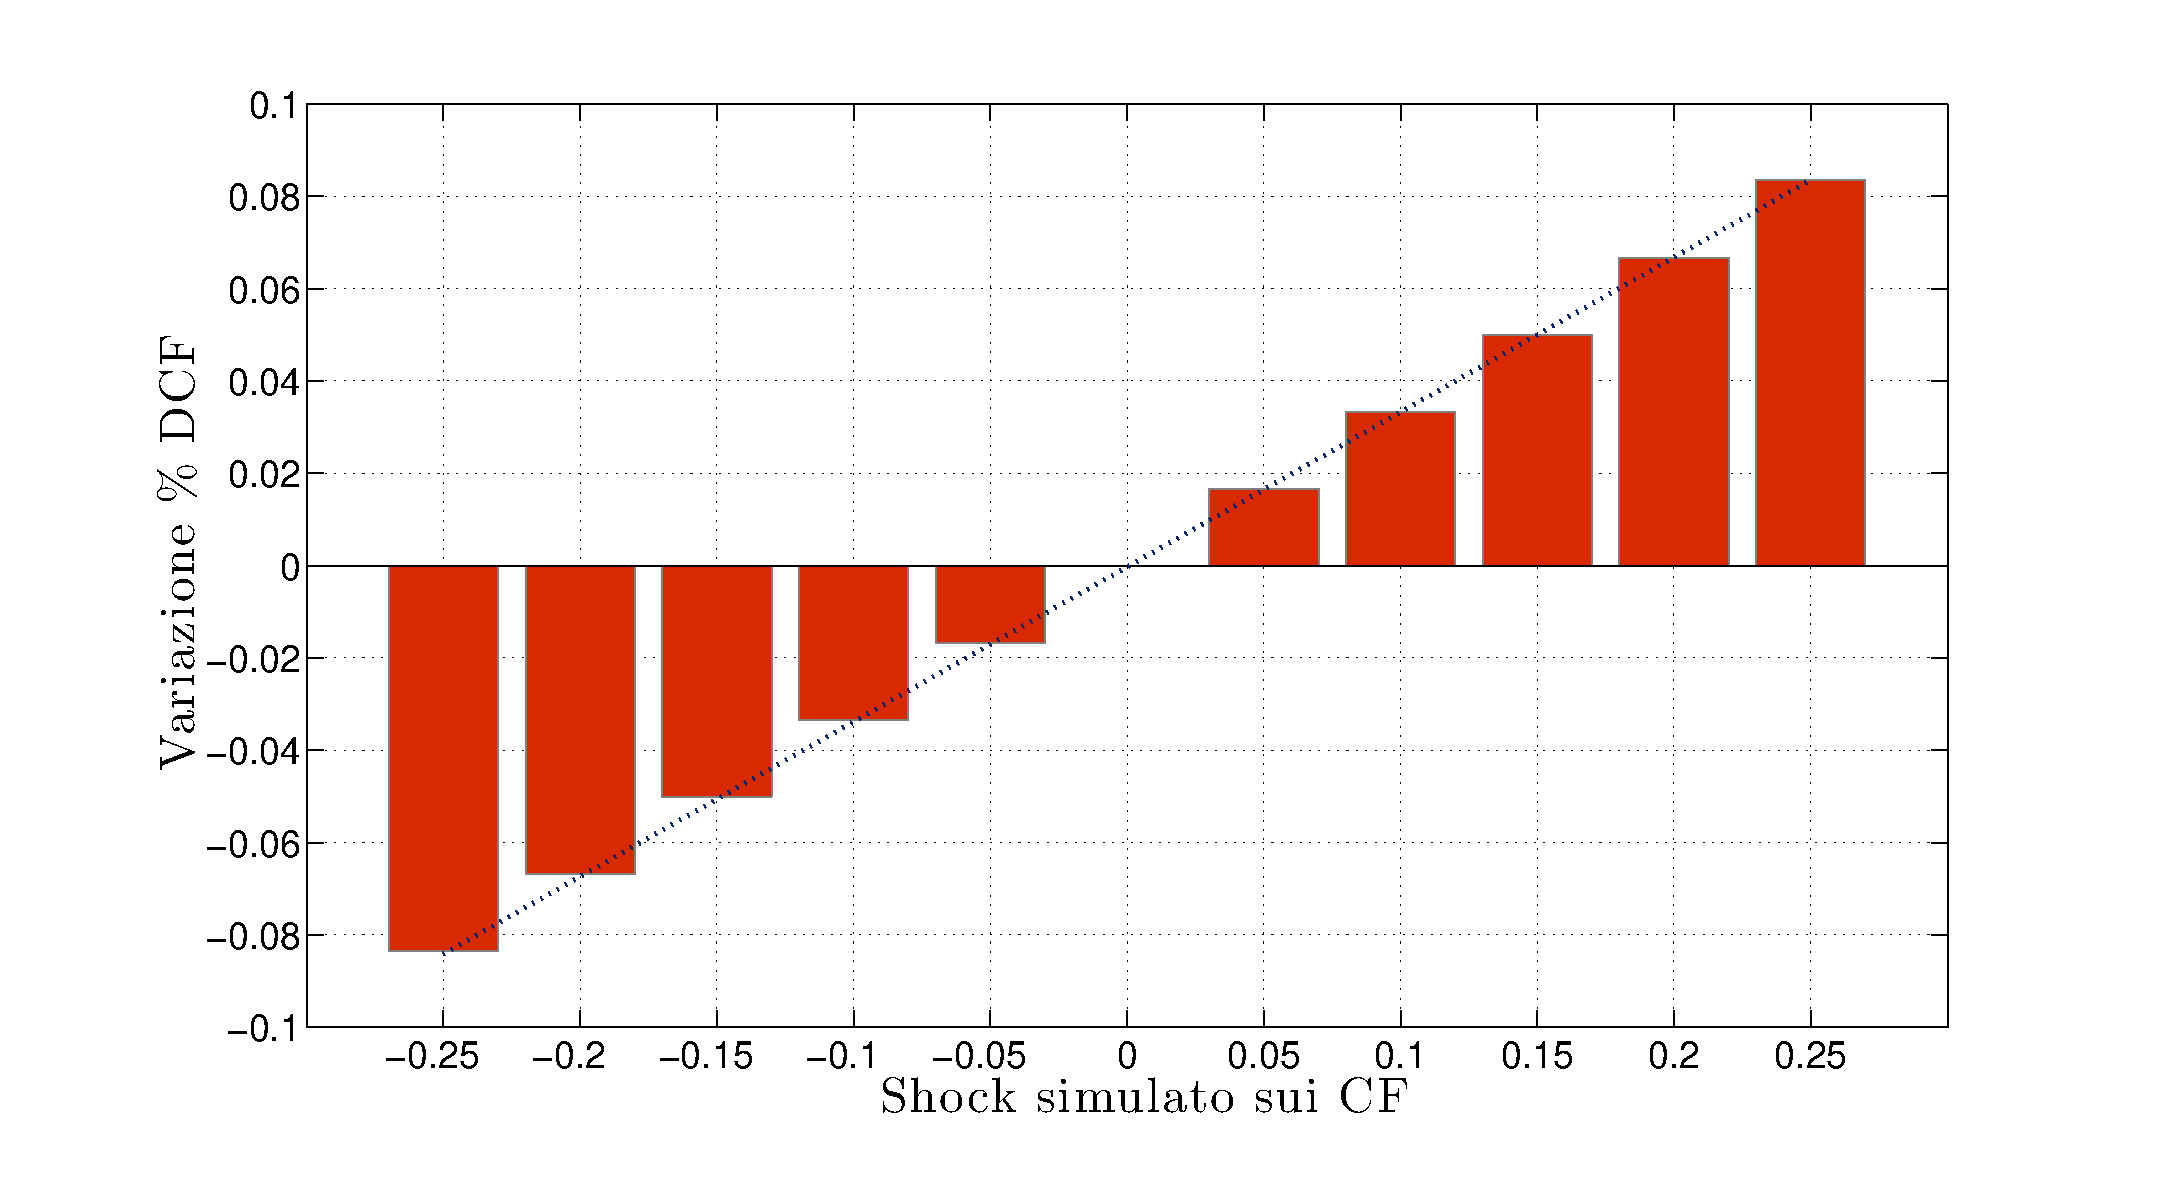
\includegraphics[scale=0.40]{Grafici/Terzo/varvcf.eps}}
\caption[Variazione media \% dei \textit{DCF} vs $\Delta$ di \textit{CF}]{Variazione percentuale media dei \textit{DCF} agli shock simulati}
\label{graf:varvcf}
\end{center}
\end{figure}

\subsection{Seconda ipotesi: shock su affitti e valore finale}
\label{subs:vcf2}
Lo scenario più probabile in caso di uno shock sulle entrate che un immobile produce è che questo coinvolga sia i canoni di locazione che l'eventuale futuro valore di cessione: in questo paragrafo si analizzano i risultati della simulazione di uno shock, quantitativamente identico al paragrafo precedente (\ref{subs:vcf1}), che coinvolge entrambe queste grandezze.
Come prevedibile, alla luce anche dei risultati della simulazione precedente, il \textit{DCF} dimostra di dipendere, per costruzione, in maniera lineare dagli importi che costituiscono i flussi di cassa. La simulazione in analisi dimostra infatti che, se lo shock impatta identicamente su canoni d'affitto e valore di cessione, il \textit{DCF} si contrae o espande del medesimo valore. La direzione del cambiamento di valore è correlata positivamente al segno dello shock. Nella tabella \ref{tab:varvcf2} sono riportati i risultati, mentre la Figura \ref{graf:varvcf2} descrive la relazione lineare unitaria fra shock e variazione della media dei \textit{DCF}. 
% Tabelle VCF Sintesi in Percentuale
\begin{table}[htbp]
\begin{center}
\begin{tabular}[c]{|c||*{4}{c|}}
\hline
$\Delta$ CF & Media & Passo & Dev Std. & Mediana \\
\hline \hline
-25\% & -25\% & -5.00\% & $\approx$ 0.00 & -25\% \\ \hline
-20\% & -20\% & -5.00\% & $\approx$ 0.00 & -20\% \\ \hline
-15\% & -15\% & -5.00\% & $\approx$ 0.00 & -15\% \\ \hline
-10\% & -10\% & -5.00\% & $\approx$ 0.00 & -10\% \\ \hline
-5\% & -5\% & -5.00\% & $\approx$ 0.00 & -5\% \\ \hline
SB & 0.00\% & 0.00\% & 0.00 & 0.00\% \\ \hline
5\% & 5\% & 5.00\% & $\approx$ 0.00 & 5\% \\ \hline
10\% & 10\% & 5.00\% & $\approx$ 0.00 & 10\% \\ \hline
15\% & 15\% & 5.00\% & $\approx$ 0.00 & 15\% \\ \hline
20\% & 20\% & 5.00\% & $\approx$ 0.00 & 20\% \\ \hline
25\% & 25\% & 5.00\% & $\approx$ 0.00 & 25\% \\ \hline
\end{tabular}
\caption[Media risultati di $\Delta$ CF e valore di cessione]{La media dei risultati delle simulazioni sulla variazione dei {\itshape cash flows} e del valore di cessione per gli immobili esaminati.}.
\label{tab:varvcf2}
\end{center}
\end{table}

% Grafico Variazione DCF vs shock CF
\begin{figure}[htbp]
\begin{center}
{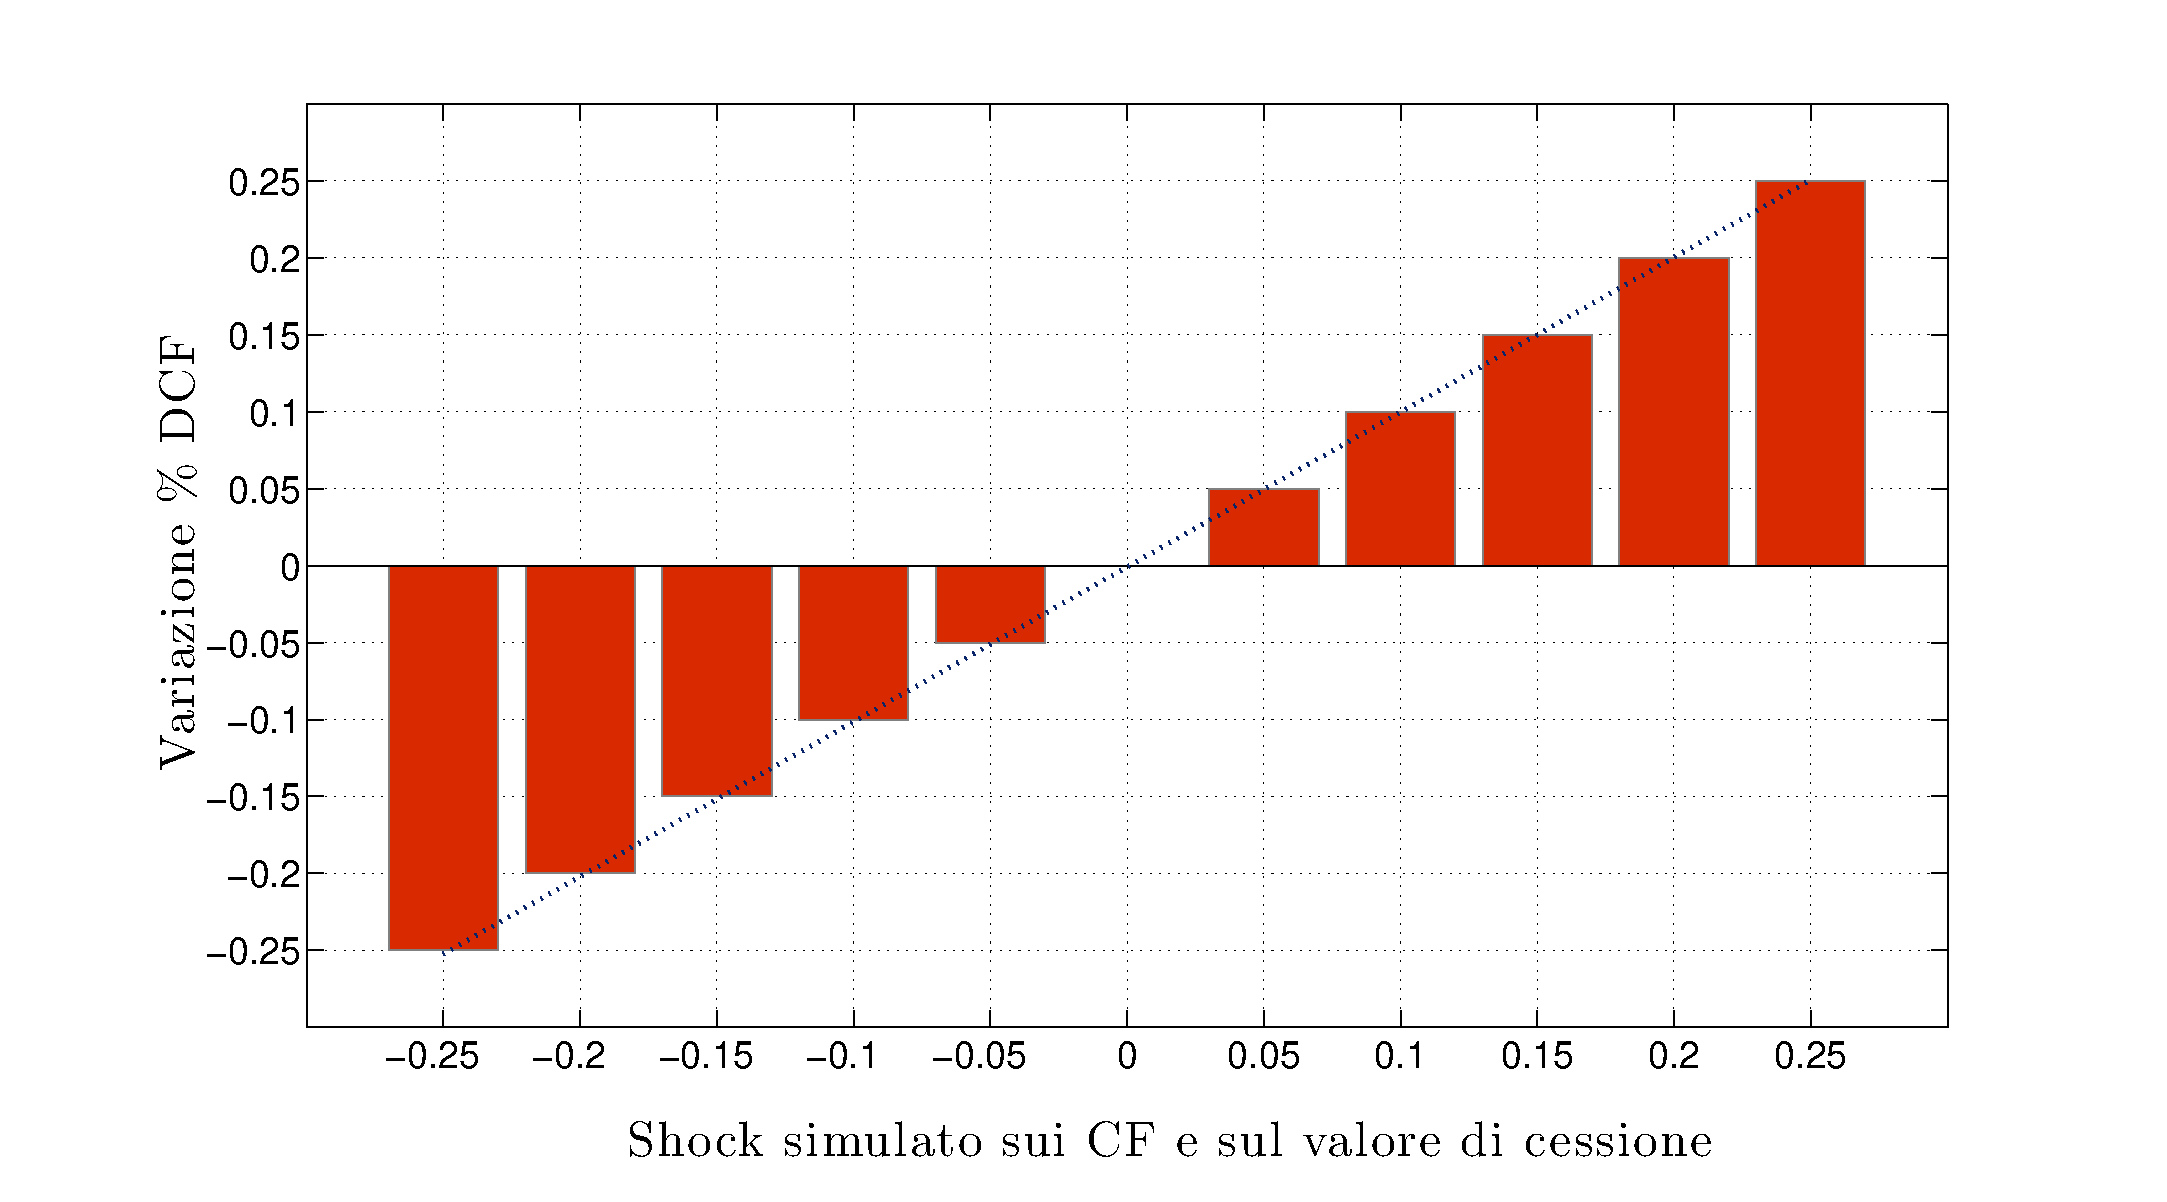
\includegraphics[scale=0.40]{Grafici/Terzo/varvcf2.eps}}
\caption[Variazione media \% dei \textit{DCF} vs $\Delta$ di \textit{CF} e valore di cessione]{Variazione percentuale media dei \textit{DCF} agli shock simulati sui \textit{CF} e sul valore di cessoine}
\label{graf:varvcf2}
\end{center}
\end{figure}

\section{Analisi dell'{\itshape interlease discount rate}}
\label{sec:simvidr}
L'{\itshape interlease discount rate} è un fattore di rischio del modello \textit{DCF} che dipende in larga misura dalla sensibilità del soggetto che compie la valutazione di un immobile. Se si osserva più da vicino la prassi del mercato immobilare si può notare che l'\textit{IDR} non viene quasi mai utilizzato, a vantaggio di un unico \textit{OCC} comprensivo anche di questa parte di rischio. Tale approccio risulta sicuramente più pratico, ma, a parità di approssimazione della stima, è meno preciso. Per questa ragione l'analisi qui svolta analizza separatamente i due tassi (per le analisi sul \textit{OCC} si veda il paragrafo \ref{sec:simvocc}), che hanno per altro una natura diversa. L'\textit{IDR} infatti mira a quantificare l'incertezza di uno o più flussi di cassa futuri, mentre l'\textit{OCC} rappresenta il tasso che si sarebbe potuto ottenere investendo diversamente il flusso di cassa.
L'ipotesi alla base dell'analisi svolta è che i primi quattro flussi di cassa siano certi, per tanto calcolati sulla base del solo \textit{OCC}, e che i successivi sei flussi siano incerti\footnote{Si ipotizza quindi che solo i primi quattro canoni di locazione siano contrattualizzati.}, quindi scontati per l'\textit{OCC} e per l'\textit{IDR}, che sconta anche il valore di cessione che viene incassato al decimo ed ultimo periodo.
Sulla scorta di questa semplice ipotesi si è svolta l'analisi di scenario che, partendo dallo scenario base, per coerenza, è stata svolta in un'unica direzione, quella positiva, in quanto per definizione l'\textit{IDR} può essere al minimo pari all'\textit{OCC}. Gli scenari ipotizzati consistono in una serie di aumenti di 100bp (1\%) a partire dal costo-opportunità del capitale che, nello scenario base è pari a 4.875\%, fino ad un {\itshape worst case scenario} del 12.875\% che rappresenta il caso limite in cui al costo-opportunità del capitale venga aggiunto un premio per il rischio dell'8\%. La scelta del valore estremo di questa magnitudo va fatta risalire all'interesse massimo sostenibile dal Paese di riferimento -- l'Italia nel caso in esame -- sui propri titoli di stato con la scadenza più simile alla struttura dell'operazione che stiamo valutando. Data questa premessa, un tal valore soglia è stato stimato da Banca d'Italia nella misura dell'8\% (\cite[p. 59]{rapportobdistabilita}) per i BTP decennali.

La tabella \ref{tab:varidrsintesi} riporta le principali statistiche descrittive ricavate dai risultati ottenuti: è di facile identificazione il comportamento della media dei \textit{DCF} che ha un andamento strettamente decrescente all'aumentare dello shock indotto sull'\textit{IDR}: ciò implica che all'aumentare dell'\textit{IDR} il valore dei \textit{DCF} si ridurrà, ma in misura sempre minore. Questo tipo di andamento è descritto graficamente dalla Figura \ref{graf:varidr}, elaborata sulla base dei risultati ottenuti nella simulazione.
% Tabelle IDR Sintesi in Percentuale
\begin{table}[htbp]
\begin{center}
\begin{tabular}[c]{|c||*{4}{c|}}
\hline
IDR & Media & Passo & Dev Std. & Mediana \\
\hline \hline
5.875\% & -30.2\% &  n.d. & 0.00583877 & -30.2\% \\ \hline
6.875\% & -34.2\% & -4.1\% & 0.00628121 & -34.3\% \\ \hline
7.875\% & -37.9\% & -3.7\% & 0.00666624 & -38.0\% \\ \hline
8.875\% & -41.3\% & -3.4\% & 0.00700058 & -41.3\% \\ \hline
9.875\% & -44.4\% & -3.1\% & 0.00729012 & -44.4\% \\ \hline
10.875\% & -47.2\% & -2.8\% & 0.00754009 & -47.2\% \\ \hline
11.875\% & -49.7\% & -2.6\% & 0.00775511 & -49.8\% \\ \hline
12.875\% & -52.1\% & -2.4\% & 0.00793922 & -52.1\% \\ \hline
\end{tabular}
\caption[Media risultati di un $\Delta^{+}$ IDR]{La media dei risultati delle simulazioni sull'aumento degli {\itshape IDR} per gli immobili esaminati.}
\label{tab:varidrsintesi}
\end{center}
\end{table}

% Grafico Variazione DCF vs shock IDR
\begin{figure}[htbp]
\begin{center}
{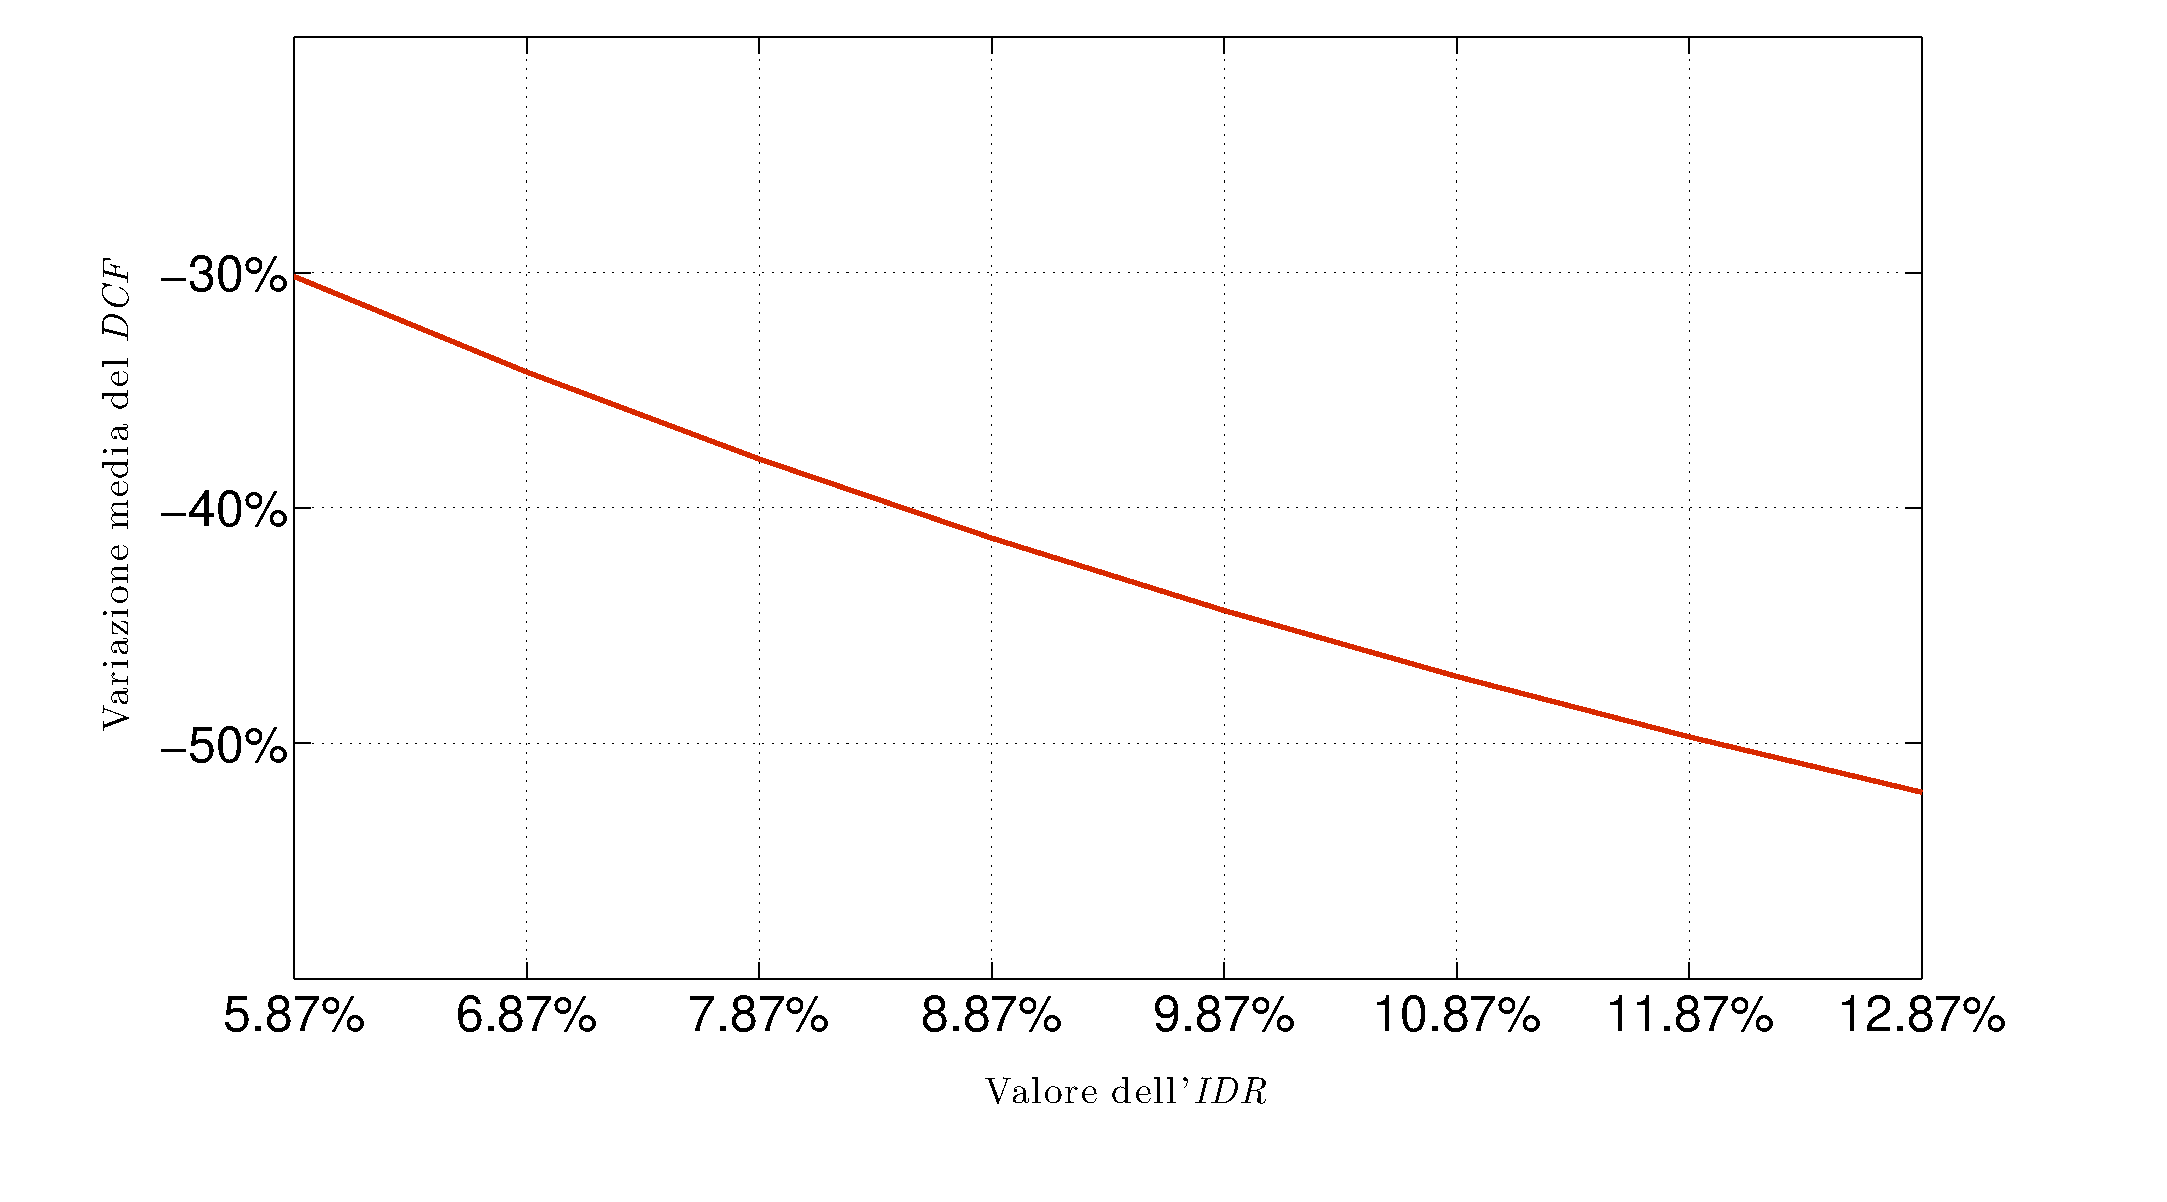
\includegraphics[scale=0.40]{Grafici/Terzo/varidr.eps}}
\caption[Variazione media \% dei \textit{DCF} vs $\Delta$ \textit{IDR}]{Variazione percentuale media dei \textit{DCF} agli shock simulati sull'\textit{IDR}}
\label{graf:varidr}
\end{center}
\end{figure}

\section{Simulazioni sul \textit{vacancy rate}}
Il {\itshape vacancy rate} è una variabile che influisce sulla {\itshape quantità di immobile} disponibili; nel caso in esame influisce sulla quantità di uffici disponibili all'interno del singolo immobile, per ipotesi stabilità in 25 unità. Il {\itshape vacancy rate} ha quindi l'effetto di ridimensionare l'ammontare dei flussi di cassa disponibili come una normale variazione dei flussi di cassa, la cui analisi è già stata svolta (in merito si veda il § \ref{sec:simvcf}).
La magnitudo degli shock è dettata dai {\itshape vacancy rate} stimati dall'\textit{IPD} che tuttavia, pur essendo l'istituzione di riferimento a livello europeo, non forniscono serie storiche per quattro delle cinque città analizzate e, per la restante (Milano), ne forniscono una poco profonda. Sulla base di ciò è stata scelta come base di partenza il 5\%\footnote{Tale dato si riferisce al primo trimestre del 2004.} che rappresenta una soglia prudenziale al di sotto del minimo rilevato nella serie storica disponibile, e come massimo il valore raggiunto da una serie  storica più profonda analoga a quella di Milano. Il dato massimo così scelto, il 12\%, è confermato anche da molti analisti di settore\footnote{Fra i vari: Scenari Immobiliari, BNP Paribas RE, CBRE.} come il valore estremo raggiungibile nei recenti anni di recessione (\cite{ilsolevacancy}, \cite[p. 3]{cbrevacancy}).
% Tabelle IDR Sintesi in Percentuale
\begin{table}[htbp]
\begin{center}
\begin{tabular}[c]{|c||*{4}{c|}}
\hline
VR & Media & Passo & Dev Std. & Mediana \\
\hline \hline
SB & 0.00\% & -1.58\% & 0.00 & 0.00\% \\ \hline
5\% & -1.58\% & -0.32\% & 0.000703832 & -1.60\% \\ \hline
6\% & -1.93\% & -0.32\% & 0.000844608 & -1.92\% \\ \hline
7\% & -2.25\% & -0.32\% & 0.000985368 & -2.25\% \\ \hline
8\% & -2.57\% & -0.32\% & 0.001126142 & -2.57\% \\ \hline
9\% & -2.89\% & -0.32\% & 0.001266908 & -2.89\% \\ \hline
10\% & -3.21\% & -0.32\% & 0.001407681 & -3.21\% \\ \hline
11\% & -3.54\% & -0.32\% & 0.001548448 & -3.53\% \\ \hline
12\% & -3.86\% & -0.32\% & 0.001689223 & -3.85\% \\ \hline
\end{tabular}
\caption[Media risultati di un $\Delta^{+}$ {\itshape vacancy rate}]{La media dei risultati delle simulazioni sulla variazione del {\itshape vacancy rate} per gli immobili esaminati.}
\label{tab:varvr}
\end{center}
\end{table}

\begin{figure}[htbp]
\begin{center}
{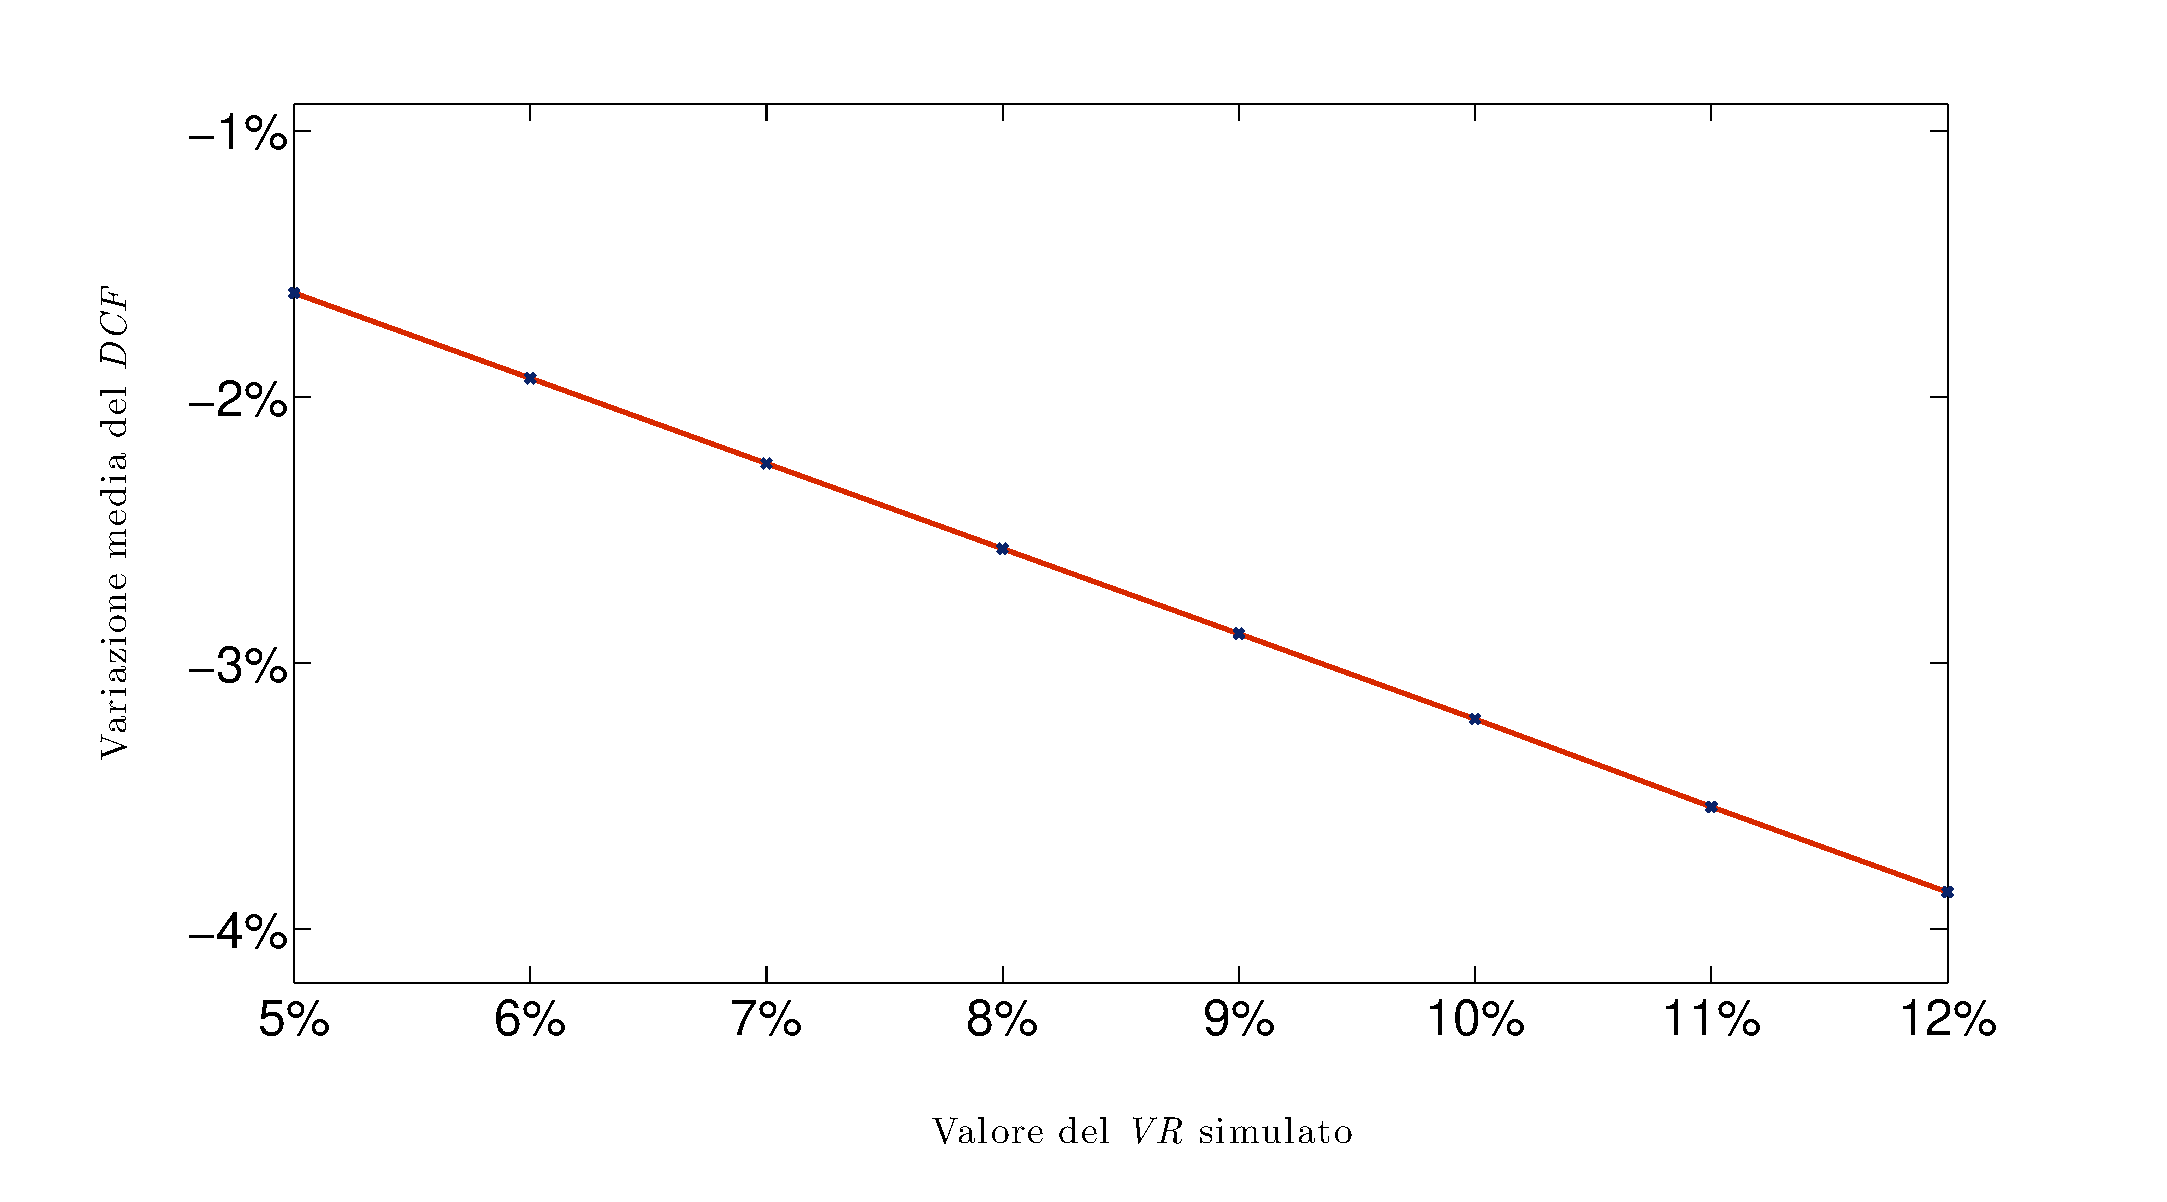
\includegraphics[scale=0.40]{Grafici/Terzo/varvr.eps}}
\caption[Variazione media \% dei \textit{DCF} vs $\Delta$ del {\itshape vacancy rate}]{Variazione percentuale media dei \textit{DCF} agli shock simulati sul {\itshape vacancy rate}}
\label{graf:varvr}
\end{center}
\end{figure}

Nella tabella \ref{tab:varvr} sono riportate le statistiche descrittive dei risultati dalle quali si può notare che la relazione fra {\itshape vacancy rate} e \textit{DCF} è lineare, così come nell'analisi dei flussi di cassa (si veda il § \ref{sec:simvcf}). Il grafico riportato in figura \ref{graf:varvr} descrive questo andamento per gli shock simulati sulla variabile.

\section{Simulazioni sull'\textit{OCC}}
\label{sec:simvocc}
Un altro \textit{driver} su cui si è svolta l'analisi di scenario è il costo-opportunità del capitale. Per questa variabile valgono alcune considerazioni svolte al paragrafo \ref{sec:simvidr}, la principale è che la scelta del tasso da applicare dipende in buona parte dalla capacità e dalla sensibilità di chi compie la valutazione. Il tasso utilizzato nello scenario base, come già descritto al § \ref{subs:risultatiscenbase}, è il tasso medio del segmento uffici dell'indice ISI. Per questa analisi di sensitività dell'\textit{OCC} è stato utilizzata una struttura dei tassi semplificata -- la medesima dello scenario base -- dove il tasso medio definito dall'ISI viene applicato a tutti i periodi: si presuppone quindi che l'immobile che si sta valutando sia, per i dieci anni in esame, sempre affittato. Nel prosieguo di questo lavoro è riportata anche un'analisi su una struttura dei tassi differente da quella semplificata qui proposta (in merito si rimanda al § \ref{subs:simvstr}).
Per la magnitudo degli shock simulati sulla variabile valgono le medesime considerazioni fatte per l'\textit{IDR} (v. \textit{supra} § \ref{sec:simvidr}), con, in aggiunta, degli scenari di diminuzione dell'\textit{OCC} progressivi di 100bp fino ad un minimo di 1.875\%.

La tabella \ref{tab:varoccsintesi} riporta le principali statistiche descrittive per scenario, ricavate dai risultati ottenuti (disponibili in valore assoluto espresso in euro nell'appendice \ref{app:risultati}, tabelle \ref{tab:rocc1} e \ref{tab:rocc2}). Anche nel caso in esame l'andamento del valore del \textit{DCF} è decrescente all'aumento dell'\textit{OCC}.

% Tabelle IDR Sintesi in Percentuale
\begin{table}[htbp]
\begin{center}
\begin{tabular}[c]{|c||*{4}{c|}}
\hline
OCC & Media & Passo & Dev Std. & Mediana \\
\hline \hline
1.875\% & 5.27\% &  1.89 & 0.00240804 & 5.25\% \\ \hline
2.875\% & 3.38\% &  1.75 & 0.00154391 & 3.37\% \\ \hline
3.875\% & 1.63\% &  1.63 & 0.00074312 & 1.62\% \\ \hline
4.875\% & 0\% &  n.d. & 0.00 & 0\% \\ \hline
5.875\% & -1.51\% &  -1.51 & 0.00069046 & -1.51\% \\ \hline
6.875\% & -2.92\% & -1.41 & 0.00133283 & -2.91\% \\ \hline
7.875\% & -4.23\% & -1.31 & 0.00193118 & -4.21\% \\ \hline
8.875\% & -5.45\% & -1.22 & 0.00248922 & -5.43\% \\ \hline
9.875\% & -6.59\% & -1.14 & 0.0030103 & -6.57\% \\ \hline
10.875\% & -7.66\% & -1.07 & 0.00349743 & -7.63\% \\ \hline
11.875\% & -8.66\% & -1.00 & 0.00395333 & -8.63\% \\ \hline
\end{tabular}
\caption[Media risultati di $\Delta$ \textit{OCC}]{La media dei risultati delle simulazioni sull'aumento dell'{\itshape OCC} per gli immobili esaminati.}
\label{tab:varoccsintesi}
\end{center}
\end{table}

% Grafico Variazione DCF vs shock OCC
\begin{figure}[htbp]
\begin{center}
{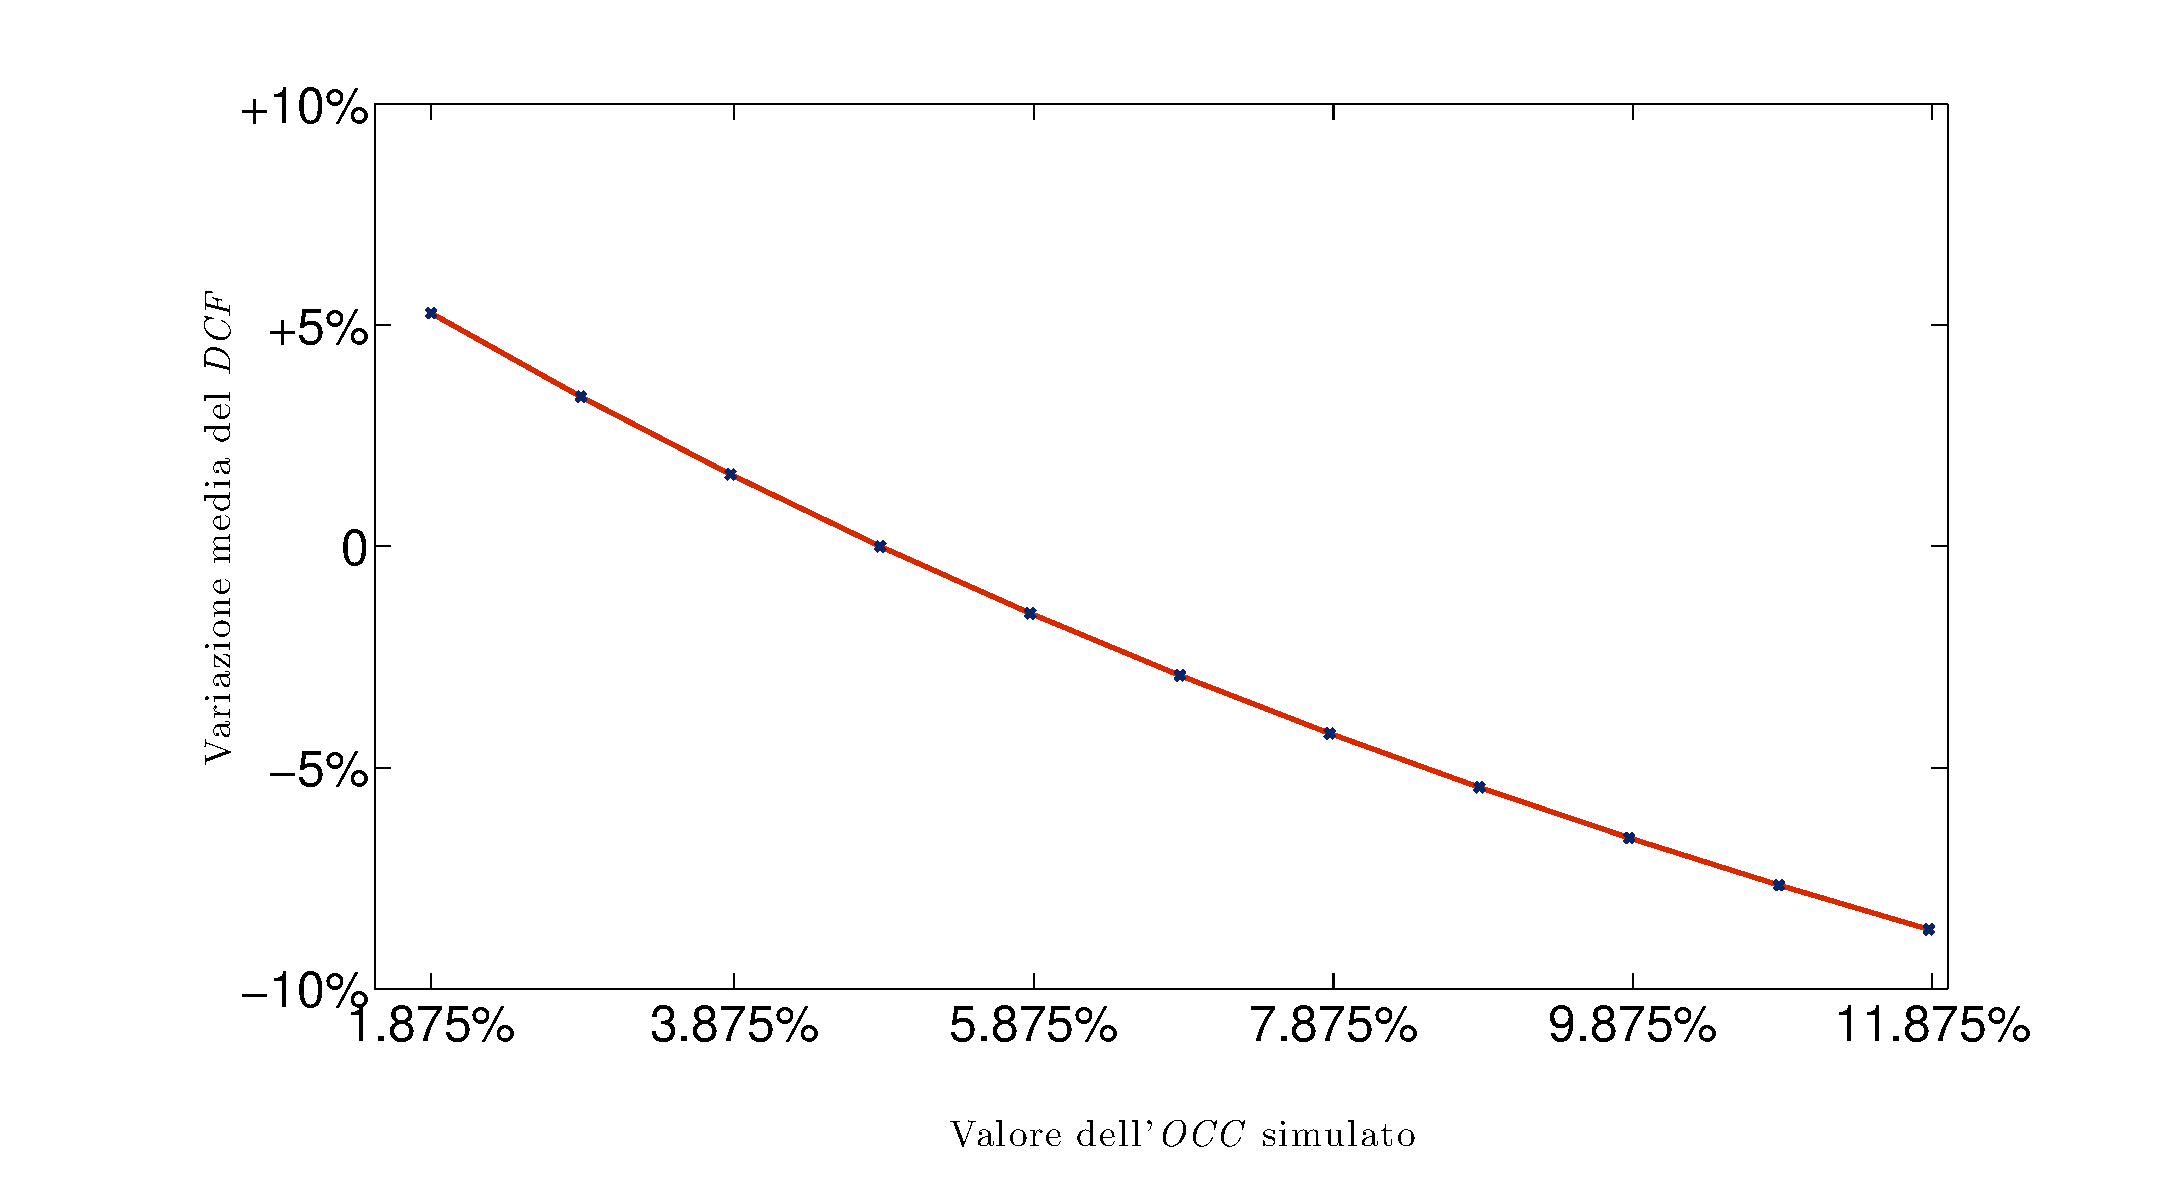
\includegraphics[scale=0.40]{Grafici/Terzo/varocc.eps}}
\caption[Variazione media \% dei \textit{DCF} vs $\Delta$ \textit{OCC}]{Variazione percentuale media dei \textit{DCF} agli shock simulati sull'\textit{OCC}}
\label{graf:varocc}
\end{center}
\end{figure}

La figura \ref{graf:varocc} descrive tale decremento, marginalmente sempre minore all'aumentare del tasso.


\subsection{Simulazioni sulla struttura dei tassi}
\label{subs:simvstr}
Un secondo tipo di analisi sull'\textit{OCC} può essere svolto ipotizzando una struttura dei tassi variabile nel tempo. In questo caso il numero di scenari ipotizzabili diventa infinito, ma è possibile identificare alcuni casi di elevato interesse pratico.

Nella continuazione dell'analisi sono stati scelti cinque scenari differenti:
\begin{enumerate}
\item un aumento annuale progressivo dell'\textit{OCC} dello 0.5\%  a partire dal tasso medio dello scenario base (4.875\%);
\item una diminuzione progressiva dello 0.5\% partendo dal 9.375\% (vale a dire l'inverso del primo scenario);
\item l'utilizzo dei tassi annuali medi degli ultimi dieci anni calcolati dall'\textit{IPD} per l'Italia;
\item uno scenario con minimi al primo e all'ultimo periodo e massimo nel periodo centrale;
\item uno scenario con massimi al primo e all'ultimo periodo e minimo nel periodo centrale.
\end{enumerate}
I risultati -- espressi in euro -- sono riportati nelle tabelle \ref{tab:rstr1} e \ref{tab:rstr2} nell'appendice \ref{app:risultati} e descritti graficamente nella figura \ref{graf:varstr}: per gli scenari in legenda è stato mantenuto l'ordine dell'elenco appena descritto. Il grafico esprime i valori, ciascuno contraddistinto da simboli, degli immobili, ordinati sull'asse delle ascisse, in ciascuno dei cinque scenari descritti. La linea azzurra descrive  un'interpolazione fra questi valori e facilita la rappresentazione dei rapporti di forza degli immobili all'interno del portafoglio immobiliare costruito. Per esemplificare, si può notare che il quinto immobile è quello con il maggior valore oppure che gli immobili dal sedicesimo al ventesimo (quelli cioè ubicati a Padova) hanno un valore omogeno fra loro, ma inferiore ai primi quattro (quelli ubicati a Milano) o alla quartina centrale (gli immobili ubicati a Torino).
\begin{sidewaysfigure}[htbp]
\begin{center}
{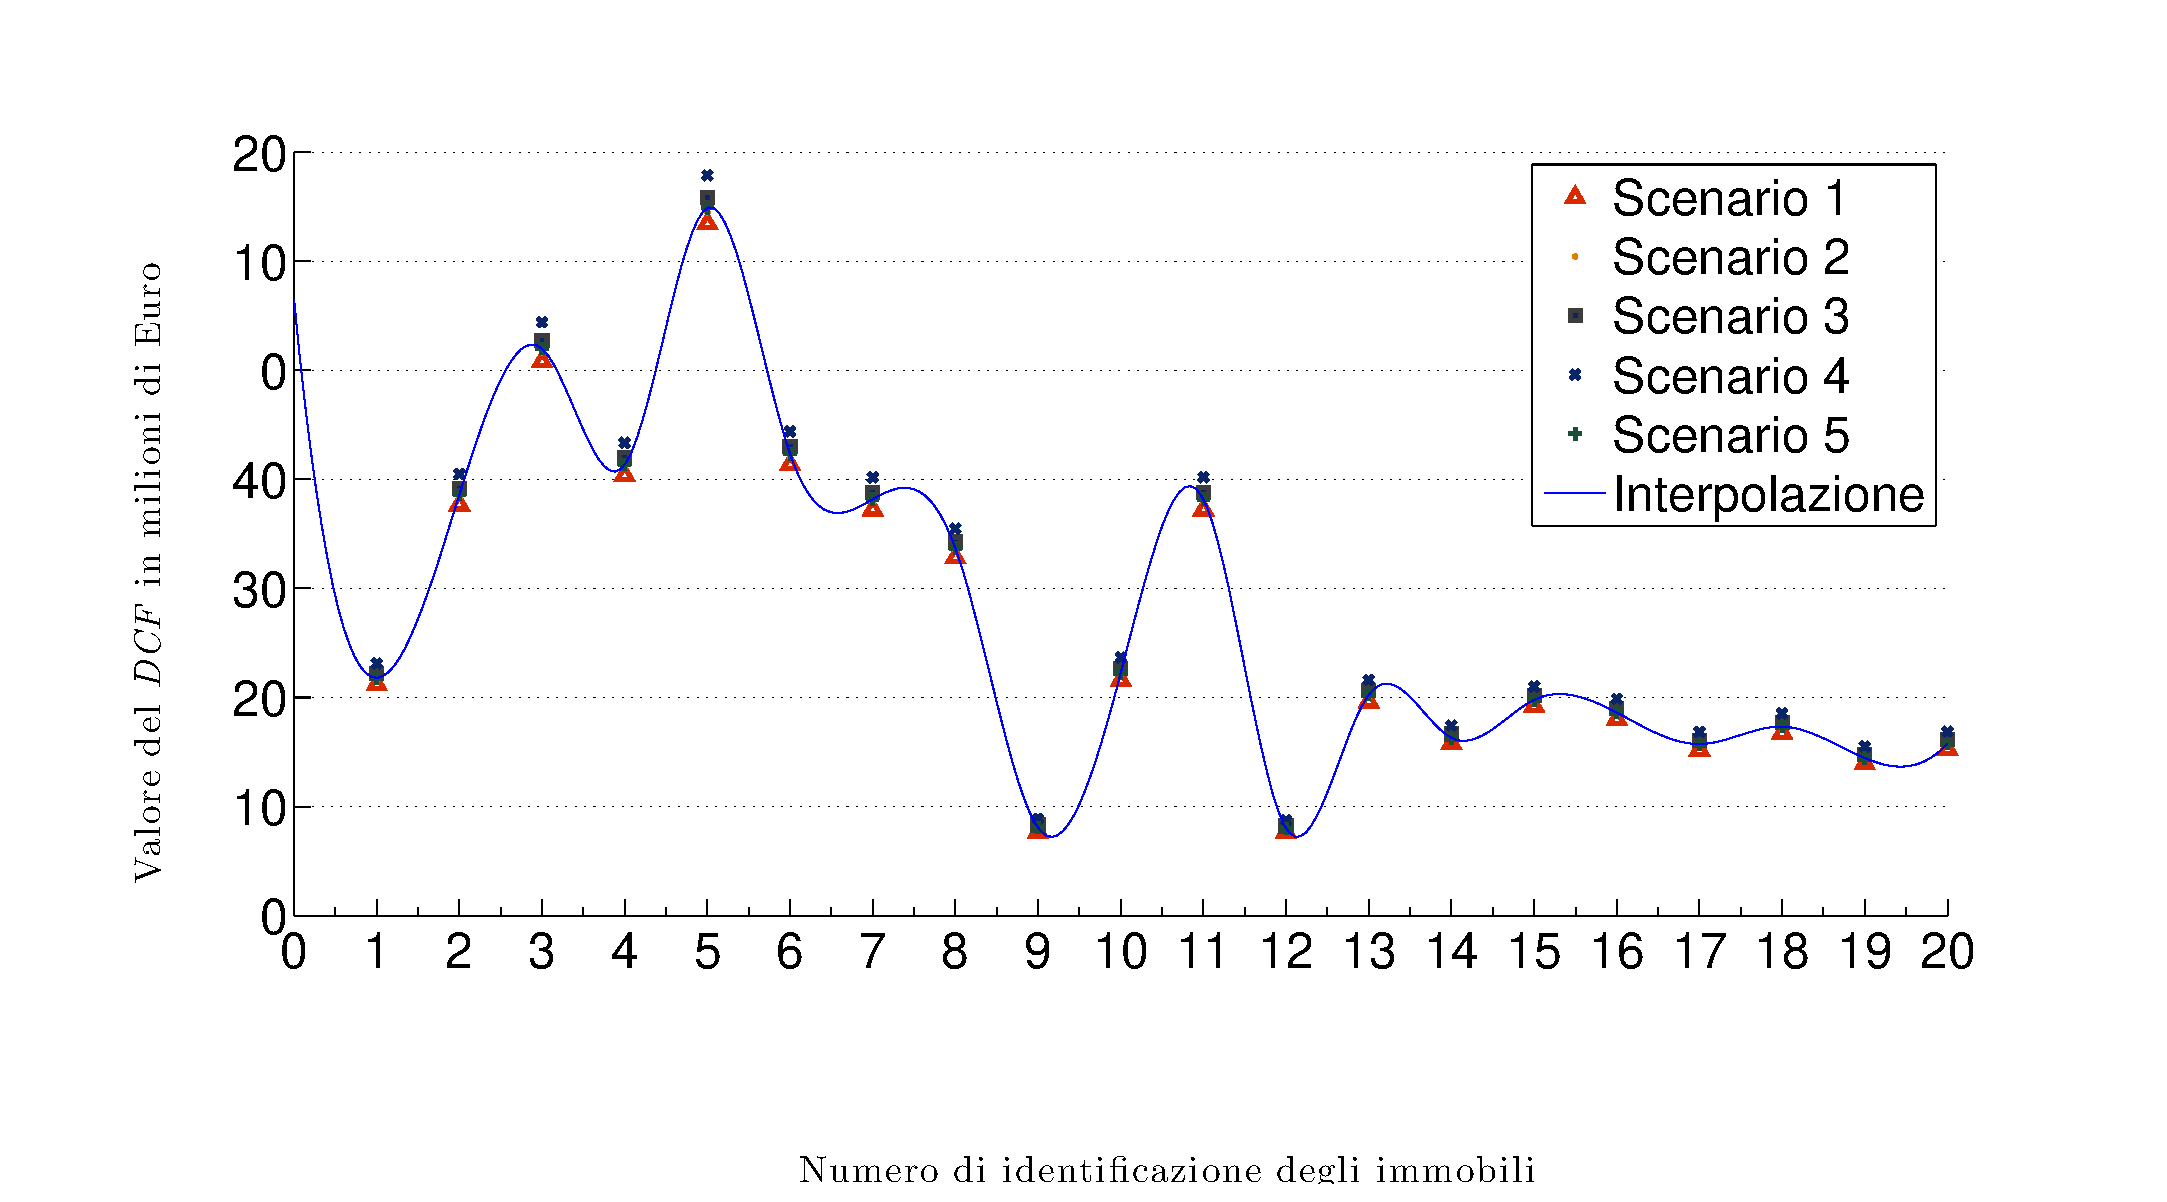
\includegraphics[scale=0.70]{Grafici/Terzo/varstr.eps}}
\caption[Confronto degli scenari di struttura dell'\textit{OCC}]{Confronto del \textit{DCF} (in \EURtm) degli immobili con cinque strutture di tassi differenti}
\label{graf:varstr}
\end{center}
\end{sidewaysfigure}

\clearpage

\section{Conclusioni}
Nel corso dell'analisi di sensitività descritta all'interno di questo capitolo si è potuto constatare che i fattori analizzati hanno un'incisività diversa sul valore finale del \textit{DCF}. 

I fattori che influiscono sull'ammontare dei flussi di cassa\footnote{Valore degli affitti, valore di cessione dell'immobile e {\itshape vacancy rate}.}, e cioè sul numeratore della formula  \ref{for:dcfinter}, incidono linearmente sull'ammontare finale del \textit{DCF} e, nello scenario più drastico, quando vi è collinearità fra shock sugli affitti e shock sul valore di cessione (§  \ref{subs:vcf1}), la riduzione percentuale del valore del \textit{DCF} è identica a quella della riduzione occorsa alla variabile.

Diversamente, la variazione dei fattori\footnote{\textit{OCC}, \textit{IDR} e, per certi tipi di analisi la struttura dei tassi} che influiscono sul denominatore della formula \ref{for:dcfinter} non ha effetti lineari sul valore dei {\itshape discount cash flows}. In questo caso ad un aumento di un fattore corrisponde una diminuzione del \textit{DCF} di portata diversa a seconda del fattore preso in analisi.
Nel caso di una simulazione univariata sull'\textit{OCC} (§ \ref{sec:simvocc}) il decremento del \textit{DCF} ha un ordine di grandezza in linea con quello dello shock ipotizzato sulla variabile, come illustrato nella tabella \ref{tab:varoccsintesi}, mentre altrettanto non avviene per un'analoga simulazione condotta sull'\textit{IDR} (§ \ref{sec:simvidr}): in questo caso infatti l'ordine di grandezza della variazione del \textit{DCF} è di circa cinque volte superiore rispetto a quello dello shock. Questo effetto è intrinseco alla costruzione del modello analizzato, che ipotizza di scontare a tassi più rischiosi, e quindi maggiori, i flussi più lontani che includono anche il valore di cessione. Possiamo dunque affermare che questa quantità è il motivo principale per cui il valore indicato dal modello \textit{DCF}\footnote{Nella versione che esplicita l'\textit{IDR} descritta alla formula \ref{for:dcfinter}} risulta così fortemente ridimensionato.

In conclusione possiamo affermare che, in un'analisi univariata, il modello dei \textit{DCF} risulta più sensibile alle variazioni dell'\textit{IDR} rispetto all'\textit{OCC}, pur non tralasciando l'importanza della scelta di una struttura dei tassi coerente con il mercato di riferimento dell'immobile -- o del portafoglio di immobili -- che si valuta. Va inoltre aggiunto che, a seconda della strategia scelta per la valutazione\footnote{Questa dipenderà dagli obiettivi e dalle eventuali norme che regolano la valutazione} e della portata degli shock, possono influenzare il valore del \textit{DCF}, in maniera apprezzabile, anche il {\itshape vacancy rate} e le altre variabili di variazione dei {\itshape cash flows}.